\documentclass[10pt]{article}
\usepackage[utf8]{inputenc}
\usepackage[english]{babel}
\usepackage[font=small,labelfont=bf]{caption}
\usepackage{geometry}
\usepackage[sort&compress, numbers, super]{natbib}
\usepackage{pxfonts}
\usepackage{graphicx}
\usepackage{setspace}
\usepackage{hyperref}
\usepackage{lineno}

\newcommand{\argmax}{\mathop{\mathrm{argmax}}\limits}

\newcommand{\demo}{S1}

\doublespacing
\linenumbers

\title{Template paper}
\author{First Author\textsuperscript{1}, Middle Author\textsuperscript{1,2}, Senior Author\textsuperscript{*, 2}\\\textsuperscript{1}Affiliation 1\\\textsuperscript{2}Affiliation 2\\\textsuperscript{*}Corresponding author: Senior.Author@university.edu}

\date{}

\begin{document}
\maketitle

\begin{abstract}
Insert abstract here
\end{abstract}


\section*{Main text}
Insert text here (Figs.~\ref{fig:demo}, \demo).

\begin{figure}[tp]
\centering
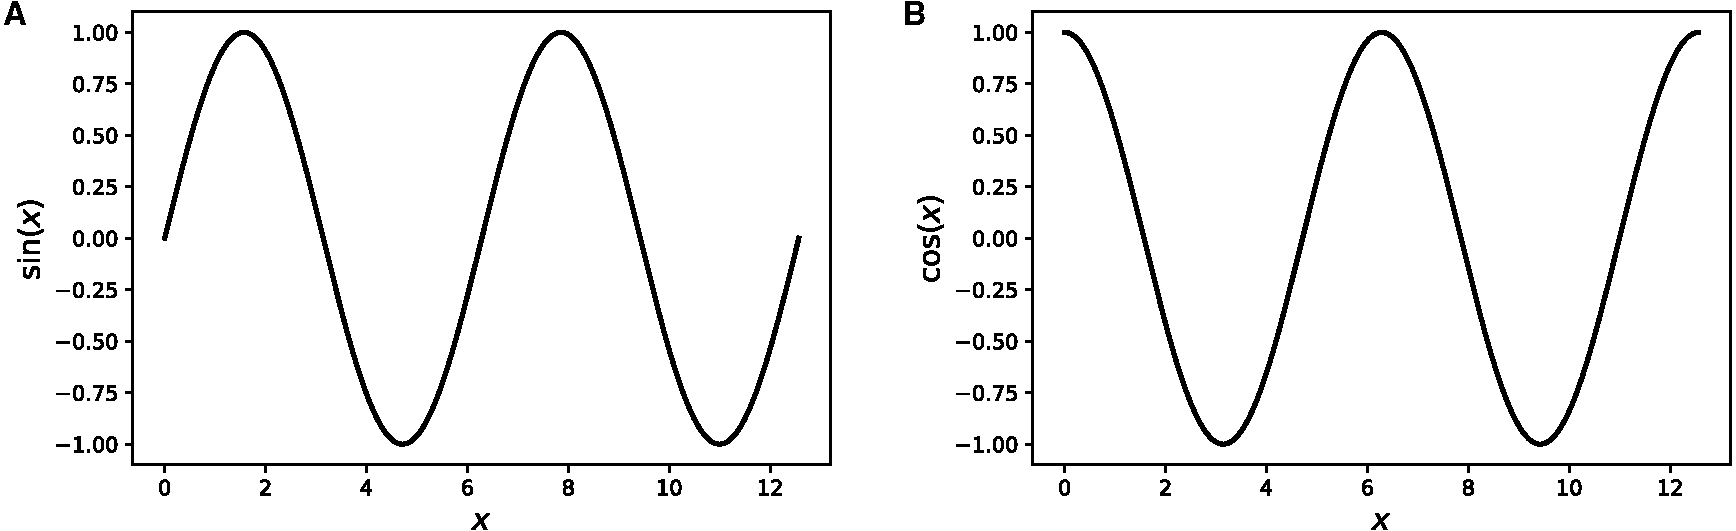
\includegraphics[width=0.8\textwidth]{figs/trig}
\caption{\textbf{Two trigonometric functions.  A. Sine wave.} Look at the pretty sine wave!  \textbf{B. Cosine wave.}  The cosine wave looks nice too.}
\label{fig:demo}
\end{figure}

\bibliographystyle{apa}
\bibliography{CDL-bibliography/cdl}
\end{document}
